\documentclass[aspectratio=169, 11pt]{beamer}

\usepackage[english]{babel}
\usepackage[T1]{fontenc}
\usepackage[default]{sourcesanspro}
\usepackage{graphicx}
\usepackage{booktabs}
\usepackage{listings}

% Same palette as the report, so the two read as one submission.
\definecolor{darkblue}{HTML}{365F91}
\definecolor{midblue}{HTML}{4F81BD}
\definecolor{ink}{HTML}{0A2333}
\definecolor{codebg}{HTML}{F4F6F8}
\definecolor{accent}{HTML}{C81E64}

\usetheme{default}
\usecolortheme{default}
\setbeamercolor{frametitle}{fg=darkblue}
\setbeamercolor{title}{fg=darkblue}
\setbeamercolor{structure}{fg=midblue}
\setbeamercolor{normal text}{fg=ink}
\setbeamertemplate{navigation symbols}{}
\setbeamertemplate{itemize item}{\color{accent}\textbullet}
\setbeamertemplate{itemize subitem}{\color{midblue}--}
\setbeamerfont{frametitle}{size=\Large, series=\bfseries}
\setbeamertemplate{footline}{%
  \hfill\tiny\color{gray}IMSE Group 05 \quad \insertframenumber/\inserttotalframenumber\hspace{2ex}\vspace{1ex}}

\lstset{
  basicstyle=\ttfamily\tiny,
  backgroundcolor=\color{codebg},
  frame=single,
  rulecolor=\color{lightgray},
  breaklines=true,
  columns=fullflexible,
  showstringspaces=false,
}

% Screenshots are 1440x900 at 2x. \shot puts one on a slide at a readable size.
\newcommand{\shot}[1]{%
  \begin{center}\includegraphics[width=0.92\textwidth,
    height=0.72\textheight, keepaspectratio]{docs/slides/#1}\end{center}}

\title{Boat Rental Company}
\subtitle{Milestone 2}
\author{Ilja Golovanov (12133820) \and Yernaz Togizbayev (01429473)}
\institute{Group 05 \quad\textbar\quad 052400-1 VU Information Management and Systems Engineering}
\date{16.06.2025}

\begin{document}

\begin{frame}[plain]
  \titlepage
\end{frame}

% ---------------------------------------------------------------- team ------
\begin{frame}{What the system does}
  A boat rental company that operates out of several harbours.
  \begin{itemize}
    \item Clients search a harbour and a date range, book a boat and pay for
          the charter
    \item Managers run the fleet, the harbours, the staff and the bookings
    \item Both analytics reports are built into the application, and both run
          against MariaDB \emph{and} MongoDB
  \end{itemize}
  \vfill
  \begin{center}
  \begin{tabular}{ll}
    \toprule
    Student 1, Ilja Golovanov     & Book a rental, availability report \\
    Student 2, Yernaz Togizbayev  & Hire a staff member, supervision report \\
    \bottomrule
  \end{tabular}
  \end{center}
\end{frame}

\begin{frame}[fragile]{Infrastructure}
  Three containers, one command.
  \begin{itemize}
    \item \textbf{db} \textendash{} MariaDB 11.3, the system of record
    \item \textbf{mongo} \textendash{} MongoDB 7, the document database
    \item \textbf{backend} \textendash{} Flask, waits for both to be healthy
  \end{itemize}
  \begin{lstlisting}[language=bash]
docker compose up --build     # then http://localhost:5000
  \end{lstlisting}
  \begin{itemize}
    \item Every dependency installed at image build, nothing needed on the host
    \item All three ports bound to \texttt{127.0.0.1}: a development server and
          two databases with known credentials do not belong on a shared network
  \end{itemize}
\end{frame}

\begin{frame}{Data import}
  \begin{columns}[T]
    \begin{column}{0.52\textwidth}
      \textbf{Generate demo data}, on every page, no login needed.
      \begin{itemize}
        \item 200 boats over every harbour, 10 clients, employees, roughly 330 rentals
        \item Boats are generated \emph{coherently}: length drives seats,
              power, weight, cabins and price
        \item Harbours are never deleted, or the only restocking tool would
              destroy every city a manager added
        \item One transaction, so a failure cannot leave it half-empty
      \end{itemize}
    \end{column}
    \begin{column}{0.48\textwidth}
      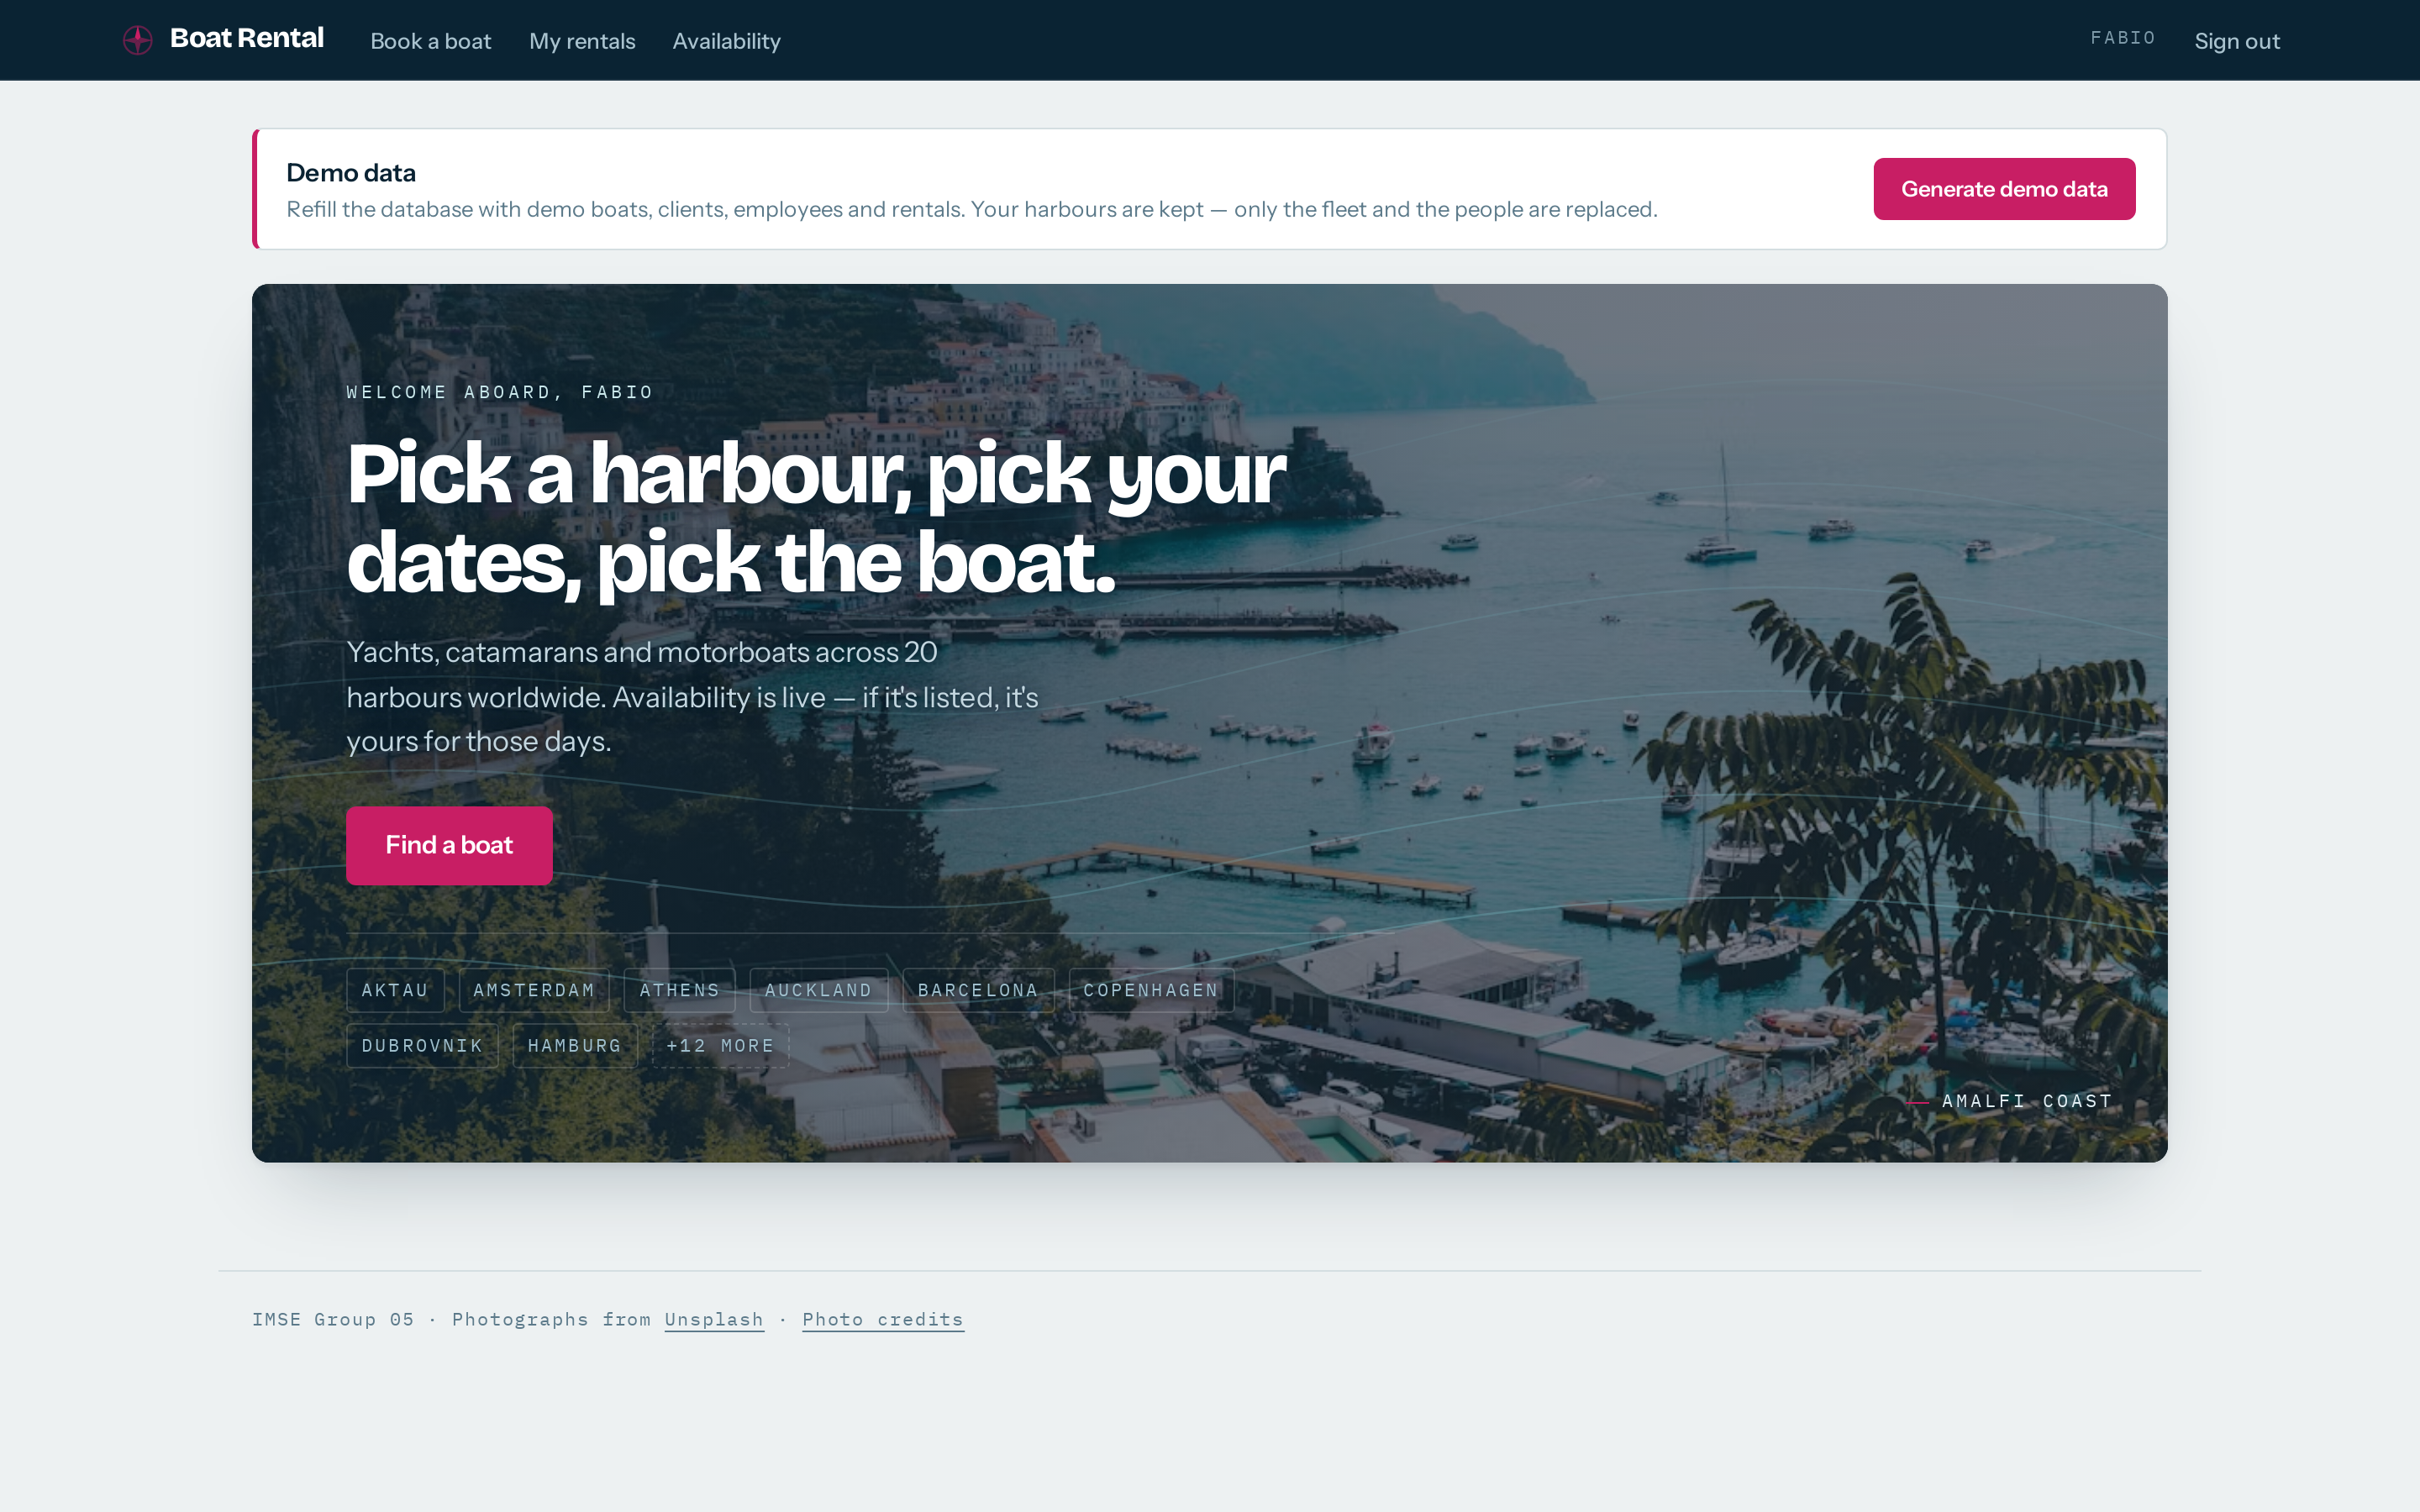
\includegraphics[width=\textwidth]{docs/slides/01-home.png}
    \end{column}
  \end{columns}
\end{frame}

% ------------------------------------------------------------ student 1 -----
\begin{frame}[plain]
  \begin{center}
    {\Large\color{darkblue}\textbf{Student 1}}\\[0.4em]
    {\large Ilja Golovanov}\\[1.2em]
    Use case: book a rental \quad\textbar\quad Report: what is free, and where
  \end{center}
\end{frame}

\begin{frame}{Use case: book a rental}
  The client picks a harbour and dates, then picks a boat.
  \shot{02-booking-results.png}
  \small The whole fleet is listed. Booked and out-of-service boats are greyed,
  labelled, and carry no radio at all, so they cannot be selected.
\end{frame}

\begin{frame}{Booking creates a hold, not a charter}
  \shot{03-checkout.png}
  \small An unpaid booking holds the boat until 24 hours before the ride. Book
  inside that window and the hold is 15 minutes, counted down live. When it
  lapses the boat goes back on the market.
\end{frame}

\begin{frame}{Analytics report: availability}
  \shot{05-availability.png}
  \small Free boats in one harbour over a date range, against the fleet size.
  Booking a boat removes it from this report: the page and the booking form
  share one overlap rule, so they cannot disagree.
\end{frame}

% ------------------------------------------------------------ student 2 -----
\begin{frame}[plain]
  \begin{center}
    {\Large\color{darkblue}\textbf{Student 2}}\\[0.4em]
    {\large Yernaz Togizbayev}\\[1.2em]
    Use case: hire a staff member \quad\textbar\quad Report: who supervises whom
  \end{center}
\end{frame}

\begin{frame}{Use case: hire a staff member}
  \shot{06-hire-staff.png}
  \small Exercises the IS-A hierarchy: one \texttt{Employee} row plus a
  \texttt{Staff} or \texttt{Manager} row. Changing someone's role later moves
  them between the two subclass tables.
\end{frame}

\begin{frame}{Analytics report: supervision}
  \shot{07-supervision.png}
  \small Which staff a manager supervises, with shift, duty status and office.
  Hiring a staff member and assigning them adds a row here: three became four.
\end{frame}

% ---------------------------------------------------------------- NoSQL -----
\begin{frame}[plain]
  \begin{center}
    {\Large\color{darkblue}\textbf{NoSQL}}\\[0.4em]
    {\large MongoDB}\\[1.2em]
    Re-design, migration, both reports, indexing
  \end{center}
\end{frame}

\begin{frame}{Re-design: shaped around the questions}
  Ten tables become three collections. Each use case's answer lives in one
  document.
  \vfill
  \begin{center}
  \begin{tabular}{lll}
    \toprule
    Collection & Embeds & Serves \\
    \midrule
    \texttt{offices}  & boats, and each boat's rentals & Student 1's report \\
    \texttt{managers} & the staff they supervise       & Student 2's report \\
    \texttt{clients}  & their own rentals              & the client logbook \\
    \bottomrule
  \end{tabular}
  \end{center}
  \vfill
  \begin{itemize}
    \item Primary keys kept as \texttt{\_id}; they are meaningful and already
          in the URLs
    \item Most foreign keys disappear: \texttt{Supervises} stops being a table,
          the relationship \emph{is} the array
    \item IS-A flattened, since nothing asks for "an employee" without knowing
          which kind
  \end{itemize}
\end{frame}

\begin{frame}[fragile]{Re-design: the trade}
\begin{lstlisting}
{ "_id": "O5", "city": "Dubrovnik", "country": "Croatia",
  "boats": [ { "boatId": "B27", "type": "catamaran", "dailyRate": "1120.00",
               "rentals": [ { "clientId": "C3", "rentalDate": "2026-09-04",
                              "paymentStatus": "PAID" } ] } ] }
\end{lstlisting}
  \begin{itemize}
    \item A rental is stored \emph{twice}, under its boat and under its client
    \item Both reads become single-document; the duplication costs nothing at
          runtime because only the migration writes
    \item It would be the first thing to revisit if the app wrote to MongoDB
          directly
  \end{itemize}
\end{frame}

\begin{frame}{Migration}
  \shot{08-nosql-console.png}
  \small One button, clears the collections first so a second run changes
  nothing. One-way: MariaDB stays the system of record. Reads through the
  existing models, so there is one definition of what a boat is.
\end{frame}

\begin{frame}[fragile]{Both reports, on documents}
  \begin{columns}[T]
    \begin{column}{0.5\textwidth}
      \textbf{Student 1} \textendash{} one aggregation
\begin{lstlisting}
db.offices.aggregate([
  { $match: { city: "Dubrovnik" } },
  { $unwind: "$boats" },
  { $match: { "boats.availabilityStatus":
              "Available" } },
  ...filter overlapping rentals...
])
\end{lstlisting}
    \end{column}
    \begin{column}{0.5\textwidth}
      \textbf{Student 2} \textendash{} one document
\begin{lstlisting}
db.managers.find({ _id: "E7" })
\end{lstlisting}
      \vspace{1em}
      \small Replaces a five-way join across \texttt{Supervises},
      \texttt{Staff}, \texttt{Employee} twice, \texttt{Manager} and
      \texttt{Office}.
    \end{column}
  \end{columns}
  \vfill
  \begin{center}
  \small\textbf{Verified, not assumed:} all 20 harbours return the same free
  boats from SQL and MongoDB, and every manager the same staff.
  \end{center}
\end{frame}

\begin{frame}{Indexing}
  \shot{09-nosql-indexes.png}
  \small \texttt{offices.city} for Student 1: 20 documents examined down to 1.
  \texttt{managers.supervisedStaff.employeeId} for the reverse of Student 2's
  report: COLLSCAN to IXSCAN. Small in absolute terms at this data size; what
  changes is that the scan grows with the collection and the lookup does not.
\end{frame}

% ----------------------------------------------------------------- close ----
\begin{frame}{Summary}
  \begin{itemize}
    \item Three containers, one command, nothing installed on the host
    \item Both use cases and both analytics reports implemented twice, on
          MariaDB and on MongoDB, and cross-checked against each other
    \item One-way migration behind a button, collections cleared first
    \item Indexes measured with \texttt{explain}, not assumed
  \end{itemize}
  \vfill
  \begin{center}\Large\color{darkblue}Questions?\end{center}
\end{frame}

\end{document}
